\documentclass{standalone}
\usepackage{tikz}
\usetikzlibrary{patterns, positioning}


\begin{document}
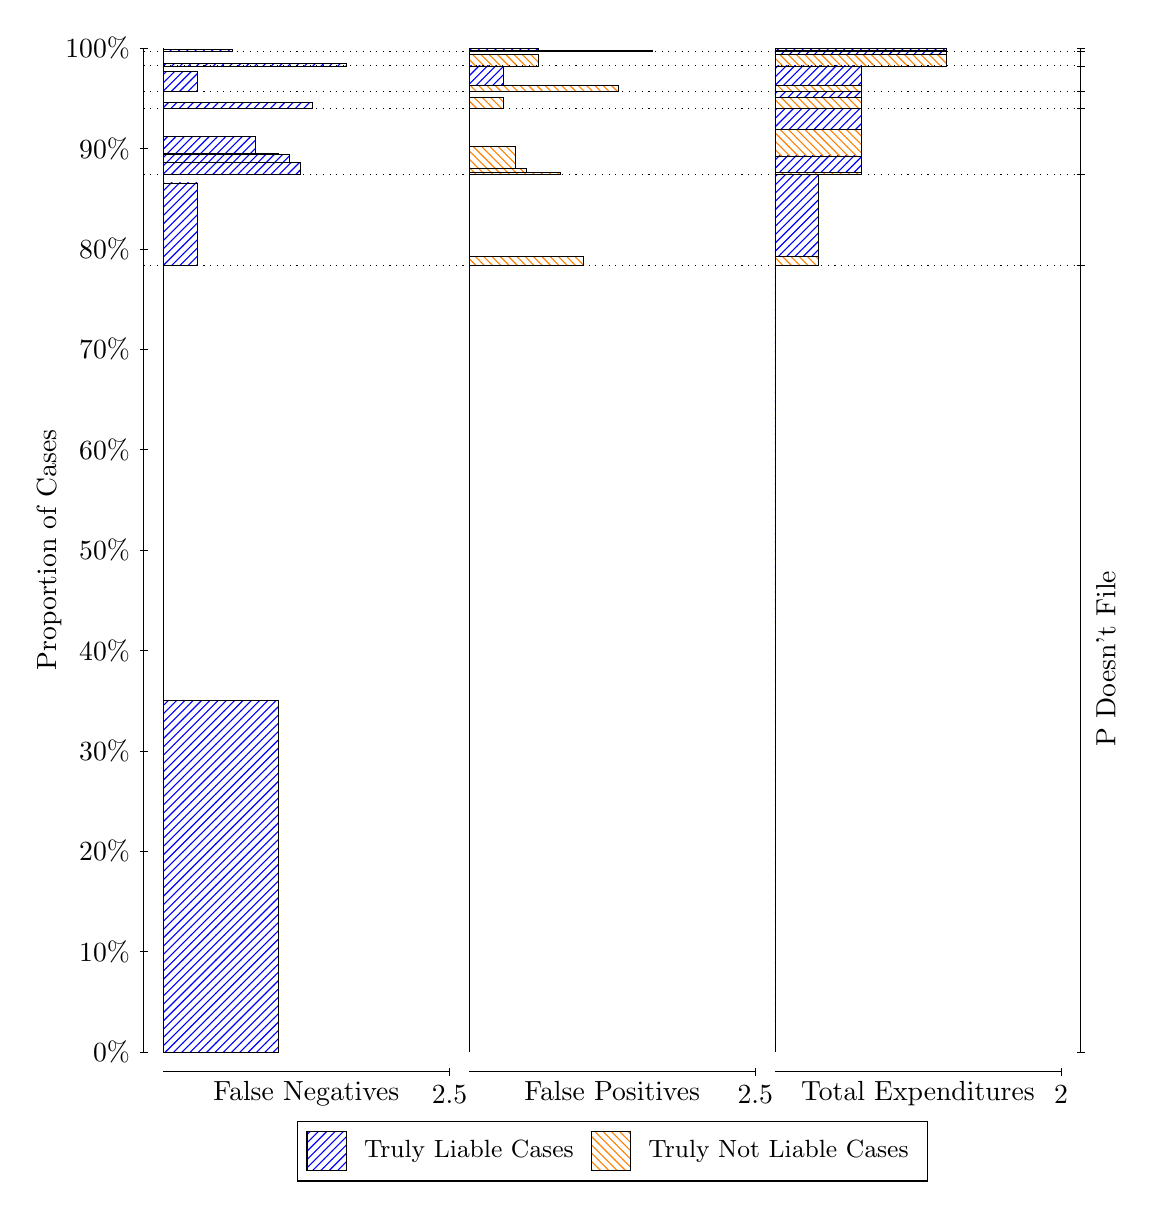
\begin{tikzpicture}
\draw[black, very thin] (1.5,1.75) -- (1.5,14.5);
\node[rotate=90, text=black, anchor=center] at (0.3, 8.125) {Proportion of Cases};
\draw[black, very thin] (1.45,1.75) -- (1.55,1.75);
\node[text=black, anchor=east] at (1.45, 1.75) {0\%};
\draw[black, very thin] (1.45,3.025) -- (1.55,3.025);
\node[text=black, anchor=east] at (1.45, 3.025) {10\%};
\draw[black, very thin] (1.45,4.3) -- (1.55,4.3);
\node[text=black, anchor=east] at (1.45, 4.3) {20\%};
\draw[black, very thin] (1.45,5.575) -- (1.55,5.575);
\node[text=black, anchor=east] at (1.45, 5.575) {30\%};
\draw[black, very thin] (1.45,6.85) -- (1.55,6.85);
\node[text=black, anchor=east] at (1.45, 6.85) {40\%};
\draw[black, very thin] (1.45,8.125) -- (1.55,8.125);
\node[text=black, anchor=east] at (1.45, 8.125) {50\%};
\draw[black, very thin] (1.45,9.4) -- (1.55,9.4);
\node[text=black, anchor=east] at (1.45, 9.4) {60\%};
\draw[black, very thin] (1.45,10.675) -- (1.55,10.675);
\node[text=black, anchor=east] at (1.45, 10.675) {70\%};
\draw[black, very thin] (1.45,11.95) -- (1.55,11.95);
\node[text=black, anchor=east] at (1.45, 11.95) {80\%};
\draw[black, very thin] (1.45,13.225) -- (1.55,13.225);
\node[text=black, anchor=east] at (1.45, 13.225) {90\%};
\draw[black, very thin] (1.45,14.5) -- (1.55,14.5);
\node[text=black, anchor=east] at (1.45, 14.5) {100\%};

\draw[black, very thin] (13.4,1.75) -- (13.4,14.5);
\draw[black, very thin] (13.35,1.75) -- (13.45,1.75);
\node[anchor=west] at (13.35, 1.75) {};
\draw[black, very thin] (13.35,11.74) -- (13.45,11.74);
\node[anchor=west] at (13.35, 11.74) {};
\draw[black, very thin] (13.35,12.899) -- (13.45,12.899);
\node[anchor=west] at (13.35, 12.899) {};
\draw[black, very thin] (13.35,13.729) -- (13.45,13.729);
\node[anchor=west] at (13.35, 13.729) {};
\draw[black, very thin] (13.35,13.952) -- (13.45,13.952);
\node[anchor=west] at (13.35, 13.952) {};
\draw[black, very thin] (13.35,14.273) -- (13.45,14.273);
\node[anchor=west] at (13.35, 14.273) {};
\draw[black, very thin] (13.35,14.453) -- (13.45,14.453);
\node[anchor=west] at (13.35, 14.453) {};
\draw[black, very thin] (13.35,14.5) -- (13.45,14.5);
\node[anchor=west] at (13.35, 14.5) {};

\draw[black, very thin, pattern color=blue, pattern=north east lines] (1.75,1.75) rectangle (3.2033,6.2161);
\draw[black, very thin, pattern color=orange, pattern=north west lines] (1.75,6.2161) rectangle (1.75,11.74);
\draw[black, very thin, pattern color=blue, pattern=north east lines] (1.75,11.74) rectangle (2.186,12.786);
\draw[black, very thin, pattern color=orange, pattern=north west lines] (1.75,12.786) rectangle (1.75,12.899);
\draw[black, very thin, pattern color=blue, pattern=north east lines] (1.75,12.899) rectangle (3.494,13.043);
\draw[black, very thin, pattern color=blue, pattern=north east lines] (1.75,13.043) rectangle (3.3487,13.15);
\draw[black, very thin, pattern color=blue, pattern=north east lines] (1.75,13.15) rectangle (3.2033,13.164);
\draw[black, very thin, pattern color=blue, pattern=north east lines] (1.75,13.164) rectangle (2.9127,13.373);
\draw[black, very thin, pattern color=orange, pattern=north west lines] (1.75,13.373) rectangle (1.75,13.729);
\draw[black, very thin, pattern color=blue, pattern=north east lines] (1.75,13.729) rectangle (3.6393,13.809);
\draw[black, very thin, pattern color=orange, pattern=north west lines] (1.75,13.809) rectangle (1.75,13.952);
\draw[black, very thin, pattern color=blue, pattern=north east lines] (1.75,13.952) rectangle (2.186,14.2);
\draw[black, very thin, pattern color=orange, pattern=north west lines] (1.75,14.2) rectangle (1.75,14.273);
\draw[black, very thin, pattern color=blue, pattern=north east lines] (1.75,14.273) rectangle (4.0753,14.305);
\draw[black, very thin, pattern color=orange, pattern=north west lines] (1.75,14.305) rectangle (1.75,14.453);
\draw[black, very thin, pattern color=blue, pattern=north east lines] (1.75,14.453) rectangle (2.622,14.481);
\draw[black, very thin, pattern color=orange, pattern=north west lines] (1.75,14.481) rectangle (1.75,14.5);
\draw[black, very thin, pattern color=orange, pattern=north west lines] (5.6333,1.75) rectangle (5.6333,7.2741);
\draw[black, very thin, pattern color=blue, pattern=north east lines] (5.6333,7.2741) rectangle (5.6333,11.74);
\draw[black, very thin, pattern color=orange, pattern=north west lines] (5.6333,11.74) rectangle (7.0867,11.853);
\draw[black, very thin, pattern color=blue, pattern=north east lines] (5.6333,11.853) rectangle (5.6333,12.899);
\draw[black, very thin, pattern color=orange, pattern=north west lines] (5.6333,12.899) rectangle (6.796,12.92);
\draw[black, very thin, pattern color=orange, pattern=north west lines] (5.6333,12.92) rectangle (6.5053,12.925);
\draw[black, very thin, pattern color=orange, pattern=north west lines] (5.6333,12.925) rectangle (6.36,12.97);
\draw[black, very thin, pattern color=orange, pattern=north west lines] (5.6333,12.97) rectangle (6.2147,13.255);
\draw[black, very thin, pattern color=blue, pattern=north east lines] (5.6333,13.255) rectangle (5.6333,13.729);
\draw[black, very thin, pattern color=orange, pattern=north west lines] (5.6333,13.729) rectangle (6.0693,13.872);
\draw[black, very thin, pattern color=blue, pattern=north east lines] (5.6333,13.872) rectangle (5.6333,13.952);
\draw[black, very thin, pattern color=orange, pattern=north west lines] (5.6333,13.952) rectangle (7.5227,14.024);
\draw[black, very thin, pattern color=blue, pattern=north east lines] (5.6333,14.024) rectangle (6.0693,14.273);
\draw[black, very thin, pattern color=orange, pattern=north west lines] (5.6333,14.273) rectangle (6.5053,14.421);
\draw[black, very thin, pattern color=blue, pattern=north east lines] (5.6333,14.421) rectangle (5.6333,14.453);
\draw[black, very thin, pattern color=orange, pattern=north west lines] (5.6333,14.453) rectangle (7.9587,14.472);
\draw[black, very thin, pattern color=blue, pattern=north east lines] (5.6333,14.472) rectangle (6.5053,14.5);
\draw[black, very thin, pattern color=orange, pattern=north west lines] (9.5167,1.75) rectangle (9.5167,7.2741);
\draw[black, very thin, pattern color=blue, pattern=north east lines] (9.5167,7.2741) rectangle (9.5167,11.74);
\draw[black, very thin, pattern color=orange, pattern=north west lines] (9.5167,11.74) rectangle (10.062,11.853);
\draw[black, very thin, pattern color=blue, pattern=north east lines] (9.5167,11.853) rectangle (10.062,12.899);
\draw[black, very thin, pattern color=orange, pattern=north west lines] (9.5167,12.899) rectangle (10.607,12.92);
\draw[black, very thin, pattern color=blue, pattern=north east lines] (9.5167,12.92) rectangle (10.607,13.129);
\draw[black, very thin, pattern color=orange, pattern=north west lines] (9.5167,13.129) rectangle (10.607,13.464);
\draw[black, very thin, pattern color=blue, pattern=north east lines] (9.5167,13.464) rectangle (10.607,13.729);
\draw[black, very thin, pattern color=orange, pattern=north west lines] (9.5167,13.729) rectangle (10.607,13.872);
\draw[black, very thin, pattern color=blue, pattern=north east lines] (9.5167,13.872) rectangle (10.607,13.952);
\draw[black, very thin, pattern color=orange, pattern=north west lines] (9.5167,13.952) rectangle (10.607,14.024);
\draw[black, very thin, pattern color=blue, pattern=north east lines] (9.5167,14.024) rectangle (10.607,14.273);
\draw[black, very thin, pattern color=orange, pattern=north west lines] (9.5167,14.273) rectangle (11.697,14.421);
\draw[black, very thin, pattern color=blue, pattern=north east lines] (9.5167,14.421) rectangle (11.697,14.453);
\draw[black, very thin, pattern color=orange, pattern=north west lines] (9.5167,14.453) rectangle (11.697,14.472);
\draw[black, very thin, pattern color=blue, pattern=north east lines] (9.5167,14.472) rectangle (11.697,14.5);
\draw[black, dotted] (1.5,11.74) -- (13.4,11.74);
\draw[black, dotted] (1.5,12.899) -- (13.4,12.899);
\draw[black, dotted] (1.5,13.729) -- (13.4,13.729);
\draw[black, dotted] (1.5,13.952) -- (13.4,13.952);
\draw[black, dotted] (1.5,14.273) -- (13.4,14.273);
\draw[black, dotted] (1.5,14.453) -- (13.4,14.453);
\draw[black, very thin] (1.75,1.5) -- (5.3833,1.5);
\node[text=black, anchor=north] at (3.5667, 1.5) {False Negatives};
\draw[black, very thin] (5.3833,1.45) -- (5.3833,1.55);
\node[text=black, anchor=north] at (5.3833, 1.45) {2.5};

\draw[black, very thin] (5.6333,1.5) -- (9.2667,1.5);
\node[text=black, anchor=north] at (7.45, 1.5) {False Positives};
\draw[black, very thin] (9.2667,1.45) -- (9.2667,1.55);
\node[text=black, anchor=north] at (9.2667, 1.45) {2.5};

\draw[black, very thin] (9.5167,1.5) -- (13.15,1.5);
\node[text=black, anchor=north] at (11.333, 1.5) {Total Expenditures};
\draw[black, very thin] (13.15,1.45) -- (13.15,1.55);
\node[text=black, anchor=north] at (13.15, 1.45) {2};

\node[text=black, centered, rotate=90] at (13.72, 6.7451) {P Doesn't File};







\draw (7.449999999999999,1.5) node[draw=none] (baseCoordinate) {};
\begin{scope}[align=center]
        \matrix[scale=0.5, draw=black, below=0.5cm of baseCoordinate, nodes={draw}, column sep=0.1cm]{
            \node[rectangle, draw, minimum width=0.5cm, minimum height=0.5cm, pattern color=blue, pattern=north east lines] {}; &
            \node[draw=none, font=\small, text=black] (B) {Truly Liable Cases}; &
            \node[rectangle, draw, minimum width=0.5cm, minimum height=0.5cm, pattern color=orange, pattern=north west lines] {}; &
            \node[draw=none, font=\small, text=black] (B) {Truly Not Liable Cases}; \\
            };
\end{scope}

\end{tikzpicture}
\end{document}